% optimization_formulation.tex  --  final formulation of the DAS / drone allocation (drones = verification layer).
% Future tense ("will be") because the report is a proposal. All numbers come from parameters_reviewed.tsv (source keys in the symbol table).
% Compile standalone (pdflatex) or copy the body (from \section) into the report. The figure s3_optimization_map.pdf is in the same folder.
% NOTE: C_total does NOT include the cost of the air-conditioned cabins: C_shelter = 0 is a PLACEHOLDER (no price was found).
\documentclass[11pt,a4paper]{article}
\usepackage[T1]{fontenc}
\usepackage{amsmath,amssymb}
\usepackage{booktabs,longtable,array}
\usepackage{graphicx}
\usepackage[margin=2.3cm]{geometry}
\newcommand{\ADzero}{\mathrm{AD}_{0}}
\newcommand{\ACzero}{\mathrm{AC}_{0}}
\newcommand{\Ctotal}{C_{\mathrm{total}}}
\newcommand{\Pzero}{P_{0}}
\newcommand{\src}[1]{\texttt{#1}}
\begin{document}

\section{Optimization of the DAS and Drone Allocation}
\label{sec:optimization}

\subsection{Roles of the sensing layers}
The Makkah boundary will be monitored by three kinds of assets. The \emph{DAS} (distributed acoustic sensing, $\Phi$-OTDR) fibre will be the only new
infrastructure; the CCTV cameras, the drones and the Point-Sensor Networks already exist in Makkah and will be used as they are, at zero capital cost.
Point-Sensor Networks are installed at the checkpoints together with the cameras, but no sensing values are available for them, so they will be excluded from
this version of the model; a switch in the code will allow them to be added later.

\paragraph{Detection} will come from the DAS and from the existing cameras only. A camera covers a short stretch of the boundary, so most of the
boundary will be detected by the DAS alone. The target is the minimum detection accuracy $\ADzero$.

\paragraph{Drones} will \emph{not} detect. They will be a \emph{response and verification} layer, which is their role in the proposed operation of the system:
a DAS alarm will steer a camera or a drone to the event, the event will be verified, and the intruder will then be tracked. There are two reasons for this choice.
First, a drone watches only a small footprint at a time and cannot supervise tens of kilometres of boundary continuously. Second, a drone is not always ready:
it will fly for $T_{d}$ minutes and then recharge for $T_{c}$ minutes. A drone will therefore be counted only for the question ``can a ready drone reach the cell
within the response time?'', and not for detection.

\paragraph{Two layers in Hot cells.} Cells will be classified as Hot, Neutral or Cold by the zoning of the digital twin. A Hot cell will need two independent layers
at every point of its boundary: a \emph{detection layer} (the DAS) and a \emph{verification layer} (a drone station that reaches the cell within the response time
with a sufficiently high probability that a drone is ready, or a camera that covers the whole cell). Neutral and Cold cells will need one layer.

\subsection{Sets and data}
The boundary will be divided into $|\mathcal{I}|=139$ cells of about $1$~km, $\mathcal{I}=\mathcal{I}_{\mathrm{Hot}}\cup\mathcal{I}_{\mathrm{Neutral}}\cup\mathcal{I}_{\mathrm{Cold}}$
with $36$, $56$ and $47$ cells. Because the fibre is continuous along the boundary, the boundary will also be cut into \emph{runs}
$\mathcal{R}$ ($|\mathcal{R}|=154$): a run is a maximal stretch of the boundary that stays inside one cell; run $r$ has length $L_r$ and $\mathcal{R}_i\subset\mathcal{R}$
is the set of runs of cell $i$. A site for an interrogator will be a run $k\in\mathcal{R}$ (the interrogator is placed on the boundary, lead-in $L_{\mathrm{lead}}=0$).
Let $\mathcal{R}_k^{+}$ and $\mathcal{R}_k^{-}$ be the runs that the right and the left channel of site $k$ can reach, i.e. whose far end is at most
$R_{\mathrm{DAS}}-L_{\mathrm{lead}}$ away along the boundary. A unit will have two active channels, one per direction, so one unit will cover at most $2R_{\mathrm{DAS}}$.
Drone stations will be chosen from a set $\mathcal{S}$ of candidate stations (boundary points every $500$~m and an interior grid every $2$~km); $\mathcal{S}_i\subset\mathcal{S}$ will be the
stations that serve cell $i$, i.e. whose distance to the farthest point of the cell is at most $R_{\mathrm{resp}}$.

The existing cameras will be placed at the road crossings of the six entrance checkpoints and of the 32 interdiction points (positions are assumed, real locations are not public).
All cameras of one site watch the same lanes, so a site will cover one stretch of $\mathrm{Cov}_{\mathrm{CCTV}}=100$~m of the boundary; $f_i\in[0,1)$ will be the fraction of the boundary of
cell $i$ covered by cameras (about $2.6\%$ of the whole boundary).

\subsection{Detection, availability and verification}
Let $p_D$ and $p_C$ be the detection probabilities of the DAS and of a camera. Intruders will be assumed to cross the cell at a uniformly distributed position, and the sensors
will be assumed to fail independently. With $x_i\in\{0,1\}$ indicating DAS fibre in cell $i$, the detection accuracy of the cell will be the length-weighted average
of $1-\prod(1-p)$ over its covered and uncovered parts, which is linear in $x_i$:
\begin{equation}
  P_{d,i}(x_i)=(1-f_i)\,x_i p_D+f_i\bigl[1-(1-x_ip_D)(1-p_C)\bigr]=f_ip_C+x_ip_D\,(1-f_ip_C).
  \label{eq:pd}
\end{equation}
A station holding $m\in\{1,\dots,K\}$ drones will have a ready drone with probability
\begin{equation}
  A(m)=\min\!\Bigl(1,\;m\,\frac{T_{d}}{T_{d}+T_{c}}\Bigr),
  \label{eq:avail}
\end{equation}
and a station will reach a cell if the farthest point of the cell lies within the response radius
\begin{equation}
  R_{\mathrm{resp}}=\min\bigl(\mathrm{Cov}_{\mathrm{drone}},\;v_{d}\,(T_{\mathrm{resp}}-T_{\mathrm{launch}})\bigr).
  \label{eq:rresp}
\end{equation}
Let $u_{s,m}\in\{0,1\}$ be $1$ if station $s$ holds $m$ drones. The probability that a drone is ready for cell $i$ will be
\begin{equation}
  A_{\mathrm{ver},i}=1-\prod_{s\in\mathcal{S}_i}\bigl(1-A(n_s)\bigr),\qquad n_s=\sum_{m}m\,u_{s,m},
  \label{eq:aver}
\end{equation}
and cell $i$ will have its verification layer if $A_{\mathrm{ver},i}\ge A_{\mathrm{ver,min}}$; the indicator is $\rho_i\in\{0,1\}$. The number of layers of cell $i$ will be
$\Lambda_i=x_i+\rho_i$ and the number required will be $\ell_i=2$ for Hot cells and $\ell_i=1$ otherwise.
To keep the problem linear, $A_{\mathrm{ver},i}$ will be evaluated on \emph{states}: the model will choose for every cell a count vector $q_i=(q_{i,1},\dots,q_{i,K})$ of drone
stations that serve it ($q_{i,m}$ stations holding $m$ drones, $\sum_mq_{i,m}\le Q$), with $A_{\mathrm{ver}}(q_i)=1-\prod_m(1-A(m))^{q_{i,m}}$ precomputed; $\rho_i=1$ if and only if $A_{\mathrm{ver}}(q_i)\ge A_{\mathrm{ver,min}}$.

\paragraph{Classification.} The classification target $\ACzero$ will be a requirement on the DAS classifier itself and will be checked once: $P_{c,\mathrm{DAS}}\ge\ACzero$. It will not be a constraint
per cell and it will not force DAS anywhere. The classification accuracy of the whole system, conditional on detection, will be computed for every cell and reported as a result. Detection succeeds if \emph{any} sensor
detects, so $1-\prod(1-p)$ is valid for detection; a classification is a decision and is right only if the (weighted) majority is right, so $1-\prod(1-p)$ will not be used for it. The sensors that detected an event,
and a verifying drone that is ready, will vote with weights $w_j=\ln\bigl(p_{c,j}/(1-p_{c,j})\bigr)$ and ties will count one half.

\subsection{Final formulation}
Let $y_k\in\{0,1\}$ indicate an interrogator at site $k$, $z_r\in\{0,1\}$ fibre on run $r$, and $a^{\pm}_{k,r}\in\{0,1\}$ that run $r\in\mathcal{R}_k^{\pm}$ is served by the right/left channel of site $k$.
Let $g_i\ge0$ and $h_i\ge0$ be the (elastic) shortfalls of the detection and of the layer requirement of cell $i$. The additional cost, with existing assets at zero cost, will be
\begin{equation}
  \Ctotal=\bigl(C_{\mathrm{DAS,int}}+C_{\mathrm{shelter}}\bigr)\sum_{k\in\mathcal{R}}y_k+C_{\mathrm{fibre}}\sum_{r\in\mathcal{R}}L_r\,z_r ,
  \label{eq:ctotal}
\end{equation}
and the objectives will be minimised in lexicographic order:
\begin{equation}
  \operatorname*{lexmin}\;\Bigl(\;N_{\mathrm{viol}},\;\;S_{\mathrm{gap}},\;\;\Ctotal,\;\;-A_{\mathrm{Hot}}\Bigr),
  \label{eq:objective}
\end{equation}
where $N_{\mathrm{viol}}=\sum_i\mathbf{1}[g_i>0\ \lor\ h_i>0]$ is the number of cells that violate a requirement, $S_{\mathrm{gap}}=\sum_i(g_i+0.1\,h_i)$ the total shortfall,
and $A_{\mathrm{Hot}}=\sum_{i\in\mathcal{I}_{\mathrm{Hot}}}A_{\mathrm{ver},i}$ the sum of the ready-probabilities over the Hot cells. The constraints will be
\begin{subequations}
\label{eq:constraints}
\begin{align}
  & P_{d,i}(x_i)+g_i\ \ge\ \ADzero, && \forall i\in\mathcal{I}, \label{eq:c-det}\\
  & x_i+\rho_i+h_i\ \ge\ \ell_i, && \forall i\in\mathcal{I}, \label{eq:c-layers}\\
  & \textstyle\sum_{m'\ge m}q_{i,m'}\ \le\ \sum_{s\in\mathcal{S}_i}\sum_{m'\ge m}u_{s,m'}, && \forall i,\ \forall m, \label{eq:c-link}\\
  & x_i\ \le\ z_r, && \forall i,\ \forall r\in\mathcal{R}_i, \label{eq:c-fibre}\\
  & a^{\pm}_{k,r_1}\le y_k,\qquad a^{\pm}_{k,r_t}\le a^{\pm}_{k,r_{t-1}},\qquad a^{\pm}_{k,r}\le z_r, && \forall k,\ r_t\in\mathcal{R}_k^{\pm}, \label{eq:c-contig}\\
  & z_r\ \le\ y_r+\textstyle\sum_{k}\bigl(a^{+}_{k,r}+a^{-}_{k,r}\bigr), && \forall r\in\mathcal{R}, \label{eq:c-service}\\
  & \textstyle\sum_{s\in\mathcal{S}}\sum_{m}m\,u_{s,m}\ \le\ N_{\mathrm{drone}},\qquad \textstyle\sum_mu_{s,m}\le1, && \forall s\in\mathcal{S}, \label{eq:c-drones}\\
  & \bigl(P_{\mathrm{DAS}}+P_{\mathrm{shelter}}\bigr)\textstyle\sum_{k}y_k\ <\ \Pzero . \label{eq:c-power}
\end{align}
\end{subequations}
Constraint~\eqref{eq:c-det} is the detection requirement of the DAS and the cameras; \eqref{eq:c-layers} requires two layers in Hot cells (DAS and verification) and one elsewhere;
\eqref{eq:c-link} lets a cell use only drone stations that exist, are within reach and hold enough drones; \eqref{eq:c-fibre}--\eqref{eq:c-service} make the fibre continuous
and installable (every fibre run will be served by an interrogator within $R_{\mathrm{DAS}}$ through fibre without gaps); \eqref{eq:c-drones} limits the drones to those that exist; and \eqref{eq:c-power}
limits the power of the new equipment, the interrogators and their air-conditioned cabins, to less than $\Pzero$.

\paragraph{Elastic constraints and the order of the objectives.} With the detection accuracy of the DAS below $\ADzero$ (for example $p_D=0.969$) or with few drones, a complete solution may not exist.
The model will therefore never be infeasible: the shortfalls $g_i,h_i$ will absorb the gap and will be reported for every cell. The solver will be run in four steps:
\begin{enumerate}
  \item minimise the number of violating cells $N_{\mathrm{viol}}$;
  \item with that number fixed, minimise the total shortfall $S_{\mathrm{gap}}$;
  \item with both fixed, minimise the additional cost $\Ctotal$;
  \item with $\Ctotal$ fixed at its minimum, maximise $A_{\mathrm{Hot}}$, i.e. place the drones where the Hot cells are verified most reliably (the drones cost nothing to us, so the cost alone would leave their positions arbitrary).
\end{enumerate}
Every step will be solved to proven optimality as a mixed-integer linear program (\texttt{intlinprog}), so the result will not depend on a heuristic.

\subsection{Algorithm steps}
\label{sec:algorithm}
The steps of the procedure, from which the flowchart in Fig.~\ref{fig:opt-flowchart} will be drawn, will be:
\begin{enumerate}
  \item Read the parameters from the parameter table; every value keeps its source or its ASSUMED / PLACEHOLDER tag.
  \item Read the cells of the digital twin (zone, length, risk) and cut the boundary into runs in the order along the boundary.
  \item Place the existing camera sites (six checkpoints matched to their roads, 32 interdiction points) and compute the covered fraction $f_i$ of every cell.
  \item Check the classifier requirement $P_{c,\mathrm{DAS}}\ge\ACzero$.
  \item Build the state table of every cell: $P_{d,i}$ from~\eqref{eq:pd}, $A_{\mathrm{ver}}$ from~\eqref{eq:aver}, layers, and the whole-system classification accuracy.
  \item Generate the candidate drone stations, compute $R_{\mathrm{resp}}$ from~\eqref{eq:rresp}, the stations that serve each cell, and remove the stations whose reach is contained in that of another.
  \item Build the sets $\mathcal{R}_k^{\pm}$ of runs that each interrogator site can reach.
  \item Build the MILP~\eqref{eq:objective}--\eqref{eq:constraints} for a scenario (3, 6 or 12 drones).
  \item Solve step 1 (fewest violating cells), then step 2 (least shortfall), step 3 (least $\Ctotal$) and step 4 (largest $A_{\mathrm{Hot}}$); print the progress (elapsed time, best solution, gap) every 10 minutes.
  \item If a verification gap remains, solve once more without the drone limit to find the fewest drones that verify every Hot cell.
  \item Recompute the verification of every cell from the final station layout, and write the per-cell table, the totals ($\Ctotal$, power against $\Pzero$, number of interrogators, drone stations) and the map.
  \item Compare with two baselines: existing assets only (no DAS), and the same drones spread evenly without optimization.
  \item Repeat for the sensitivity cases ($p_D$, $P_{c,\mathrm{DAS}}$, $T_{\mathrm{resp}}$, $A_{\mathrm{ver,min}}$, $C_{\mathrm{fibre}}$).
\end{enumerate}

\begin{figure}[ht]
  \centering
  \fbox{\parbox{0.8\linewidth}{\centering\vspace{3cm}The flowchart of the steps in Section~\ref{sec:algorithm} will be drawn here.\vspace{3cm}}}
  \caption{Flowchart of the optimization procedure (to be drawn from the algorithm steps).}
  \label{fig:opt-flowchart}
\end{figure}

\begin{figure}[ht]
  \centering
  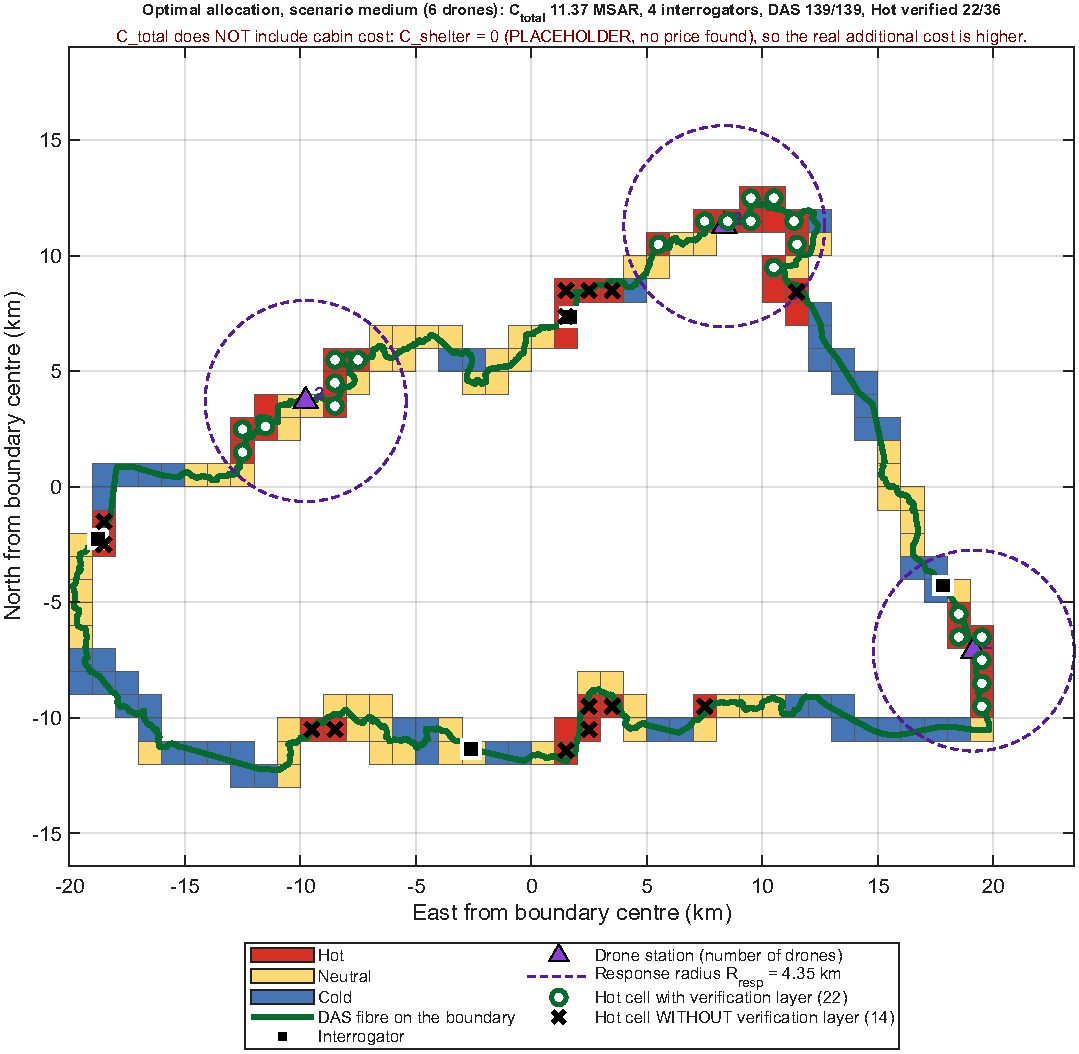
\includegraphics[width=\linewidth]{s3_optimization_map.pdf}
  \caption{Optimal allocation for the medium scenario (6 drones): DAS fibre on the boundary, interrogators, drone stations with their response circles, and the Hot cells with and without a verification layer.
  $\Ctotal$ does not include the cost of the cabins ($C_{\mathrm{shelter}}=0$, PLACEHOLDER).}
  \label{fig:s3-map}
\end{figure}

\subsection{Assumptions and limits}
\begin{itemize}
  \item Sensors will be assumed to fail independently; this may be optimistic because they share weather and terrain.
  \item The intruder position will be assumed uniform along the cell; existing cameras will cover one $100$~m stretch per site.
  \item A drone station will be assumed to serve every cell in its reach; simultaneous alarms in different cells are not modelled.
  \item Drone stations will be chosen from a candidate set because the real dock sites are not public.
  \item $C_{\mathrm{shelter}}=0$ is a PLACEHOLDER, so $\Ctotal$ will be lower than the real additional cost; $C_{\mathrm{fibre}}$ has no published Saudi source and will be varied by $\times0.5$ and $\times2$.
  \item $T_{\mathrm{resp}}$ and $A_{\mathrm{ver,min}}$ are PLACEHOLDERs; $T_{\mathrm{launch}}$ comes from a reseller page and must be verified on the manufacturer page.
\end{itemize}

\subsection{Symbols}
\begin{longtable}{@{}p{2.9cm}p{5.6cm}p{3.2cm}p{3.6cm}@{}}
\caption{Symbols, values and sources (every value is in the parameter table; the source keys are BibTeX keys).}\label{tab:symbols}\\
\toprule
Symbol & Meaning & Value & Source key / tag \\ \midrule
\endfirsthead
\toprule Symbol & Meaning & Value & Source key / tag \\ \midrule
\endhead
\bottomrule
\endfoot
$\ADzero$ & minimum detection accuracy of every cell & $0.98$ & project target \\
$\ACzero$ & minimum classification accuracy (check on the DAS classifier) & $0.98$ & project target \\
$\Pzero$ & upper limit of the power of the new equipment & $29{,}100$~W & CCTV-only system, $1455\times20$~W \\
$\Ctotal$ & additional cost (objective), without cabins & result & --- \\
$\mathcal{I}$, $\mathcal{R}$, $\mathcal{S}$ & cells, boundary runs, candidate drone stations & $139$, $154$, $457$ & DAS-map; ASSUMED \\
Hot / Neutral / Cold & zones of the cells & $36$ / $56$ / $47$ cells & DAS-map zoning \\
$L_r$ & length of run $r$ & about $1$~km (cell size) & DAS-map \\
$f_i$ & fraction of cell $i$ covered by existing cameras & computed ($2.6\%$ overall) & ASSUMED positions \\
$\mathrm{Cov}_{\mathrm{CCTV}}$ & boundary stretch covered by one camera site & $100$~m & table row \\
checkpoints / cameras & entrance checkpoints, cameras per checkpoint & $6$, $16$ & \src{alwatan\_checkpoints}, \src{okaz\_shumaisi} \\
interdiction points & number, cameras per point & $32$, $4$ (PLACEHOLDER) & \src{ajel\_32points} \\
$p_D$ & detection probability of the DAS & $0.969$ (sens.\ $0.98$, $1.0$) & \src{zeng2024}, \src{liu2016} \\
$p_C$ & detection probability of a camera & $0.909$ & table row (Park et al.) \\
$P_{c,\mathrm{DAS}}$ & classification accuracy of the DAS classifier & $0.983$--$0.993$ & \src{wang2024} \\
$p_{c,C}$, $p_{c,\mathrm{drone}}$ & classification accuracy of a camera, of a drone & $0.85$, $0.89$ (proxy) & table row; \src{khan\_uav\_thermal} \\
$R_{\mathrm{DAS}}$ & sensing range of one channel & $20$~km & FEBUS A1-NEO datasheet \\
$L_{\mathrm{lead}}$ & lead-in fibre from the cabin to the boundary & $0$~m & ASSUMED \\
$P_{\mathrm{DAS}}$, $P_{\mathrm{shelter}}$ & power of one interrogator, of its cabin cooling & $170$~W, $170$~W & datasheet; \src{gsma\_coolsure} \\
$C_{\mathrm{DAS,int}}$ & cost of one interrogator & $636{,}000$~SAR & vendor meeting, FX assumed \\
$C_{\mathrm{shelter}}$ & cost of one cabin & $0$ (not costed) & PLACEHOLDER \\
$C_{\mathrm{fibre}}$ & cost of fibre with installation & $60{,}700$~SAR/km & PLACEHOLDER (sens.\ $\times0.5$, $\times2$) \\
$N_{\mathrm{drone}}$ & drones available (low / medium / high) & $3$ / $6$ / $12$ & ASSUMED; \src{yenisafak2026drones} \\
$T_{d}$, $T_{c}$ & flight time, recharge time of a drone & $47$~min, $27$~min & table row; \src{dji\_dock3\_specs} \\
$v_{d}$ & maximum horizontal speed (Dock mode) & $15$~m/s & \src{dji\_dock3\_specs} \\
$T_{\mathrm{launch}}$ & takeoff time from the dock & $10$~s & \src{advexure\_dock3} (reseller, VERIFY) \\
$T_{\mathrm{resp}}$ & required response time & $300$~s (sens.\ $180$, $600$) & PLACEHOLDER \\
$\mathrm{Cov}_{\mathrm{drone}}$ & operating radius of a drone & $11$~km & table row \\
$R_{\mathrm{resp}}$ & response radius, eq.~\eqref{eq:rresp} & $4350$~m & derived \\
$A_{\mathrm{ver,min}}$ & minimum probability that a drone is ready & $0.9$ (sens.\ $0.8$, $0.95$) & PLACEHOLDER \\
$K$, $Q$ & most useful drones per station, most stations serving one cell & $2$, $2$ & derived; ASSUMED \\
$C_{\mathrm{drone}}$ & price of a drone with its dock (reference only) & $148{,}887$~SAR & table row \\
\end{longtable}

\end{document}
